\section{Results}
% Tables and figures summarizing all tasks.
% Highlight trade-offs: performance vs. efficiency vs. stability.
\subsection{Before Permutation}
For the graph classification tasks before any pertubation, we present the performance of each embedding method across the three TUDatasets with  accuracy, F1-score and AUC metrics for each method in Tables~\ref{tab:gin_best}, ~\ref{tab:graph2vec_best} and ~\ref{tab:netlsd_best}. 
% along with computational metrics such as training time and memory usage.
We preferered to show only the best test configuration per dataset x dim results and for the epochs 200 and 300 (for GIN) for the reason we mentioned in earlier section.


\begin{table}[t]
\centering
\caption{GIN classification performance on EMB1 datasets (epochs $\in\{200,300\}$). Best configuration per embedding dimension is reported.}
\label{tab:gin_best}
\begin{tabular}{l c c c c c}
\hline
\textbf{Dataset} & \textbf{Dim} & \textbf{Epochs} & \textbf{Acc} & \textbf{F1} & \textbf{AUC} \\
\hline
MUTAG      & 64  & 200 & 0.842 & 0.825 & 0.885 \\
MUTAG      & 128 & 200 & 0.842 & 0.808 & 0.885 \\
MUTAG      & 256 & 200 & 0.895 & 0.864 & 0.859 \\
\hline
ENZYMES    & 64  & 300 & 0.433 & 0.428 & 0.703 \\
ENZYMES    & 128 & 300 & 0.483 & 0.492 & 0.744 \\
ENZYMES    & 256 & 300 & 0.617 & 0.615 & 0.809 \\
\hline
IMDB-MULTI & 64  & 200 & 0.500 & 0.496 & 0.686 \\
IMDB-MULTI & 128 & 200 & 0.500 & 0.486 & 0.678 \\
IMDB-MULTI & 256 & 200 & 0.507 & 0.478 & 0.714 \\
\hline
\end{tabular}
\end{table}


\begin{table}[t]
\centering
\caption{Best Graph2Vec classification results per dataset and embedding dimension. 
For each dataset--dimension pair, the classifier with the highest test accuracy is reported.}
\label{tab:graph2vec_best}
\begin{tabular}{l c c c c c}
\hline
\textbf{Dataset} & \textbf{Dim} & \textbf{Model} & \textbf{Acc} & \textbf{F1} & \textbf{AUC} \\
\hline
MUTAG      & 64  & RF  & 0.711 & 0.656 & 0.775 \\
MUTAG      & 128 & RF  & 0.763 & 0.754 & 0.797 \\
MUTAG      & 256 & RF  & 0.737 & 0.731 & 0.745 \\
\hline
ENZYMES    & 64  & Ens & 0.258 & 0.252 & 0.571 \\
ENZYMES    & 128 & RF  & 0.225 & 0.219 & 0.600 \\
ENZYMES    & 256 & RF  & 0.317 & 0.310 & 0.591 \\
\hline
IMDB-MULTI & 64  & RF  & 0.437 & 0.435 & 0.601 \\
IMDB-MULTI & 128 & GB  & 0.427 & 0.426 & 0.583 \\
IMDB-MULTI & 256 & SVM & 0.433 & 0.426 & 0.599 \\
\hline
\end{tabular}
\end{table}



\begin{table}[t]
\centering
\caption{Best NetLSD classification results per dataset and embedding dimension. 
For each dataset--dimension pair, the classifier with the highest test accuracy is reported.}
\label{tab:netlsd_best}
\begin{tabular}{l c c c c c}
\hline
\textbf{Dataset} & \textbf{Dim} & \textbf{Model} & \textbf{Acc} & \textbf{F1} & \textbf{AUC} \\
\hline
MUTAG      & 64  & Ens & 0.895 & 0.892 & 0.908 \\
MUTAG      & 128 & Ens & 0.868 & 0.867 & 0.883 \\
MUTAG      & 256 & LR  & 0.868 & 0.867 & 0.929 \\
\hline
ENZYMES    & 64  & RF  & 0.300 & 0.302 & 0.666 \\
ENZYMES    & 128 & RF  & 0.308 & 0.312 & 0.653 \\
ENZYMES    & 256 & RF  & 0.325 & 0.324 & 0.673 \\
\hline
IMDB-MULTI & 64  & SVM & 0.480 & 0.477 & 0.625 \\
IMDB-MULTI & 128 & RF  & 0.463 & 0.465 & 0.633 \\
IMDB-MULTI & 256 & RF  & 0.457 & 0.456 & 0.648 \\
\hline
\end{tabular}
\end{table}

For the MUTAG, we can see that GIN excels in classification accuracy, but NetLSD provides 
superior probabilistic separation as indicated by its higher AUC scores. 
AUC slightly decreases with increasing dimensions for GIN, showing that 
higher classification accuray does not always mean that the method 
has confidence in its predictions. 
So, our conclusion is that spectral info captured by NetLSD is beneficial for this dataset.
For ENZYMES, the gap between GIN and the other two methods is clearer in all metrics.
GIN clearly dominates here and AUC metric confirms that GIN is more confident in its predictions.
For IMDB-MULTI, when node features are absent, GIN and NetLSD have similar behavior, with GIN slightly ahead.

So overall, GIN is the most effective method and NetLSD is second best, 
while Graph2Vec shows the weakest performance across all datasets and metrics.
The results confirm that supervised GNNs provide the highest predictive power, while spectral descriptors such as 
NetLSD remain surprisingly strong for unsupervised graph representation learning.

\begin{figure}[t]
    \centering
    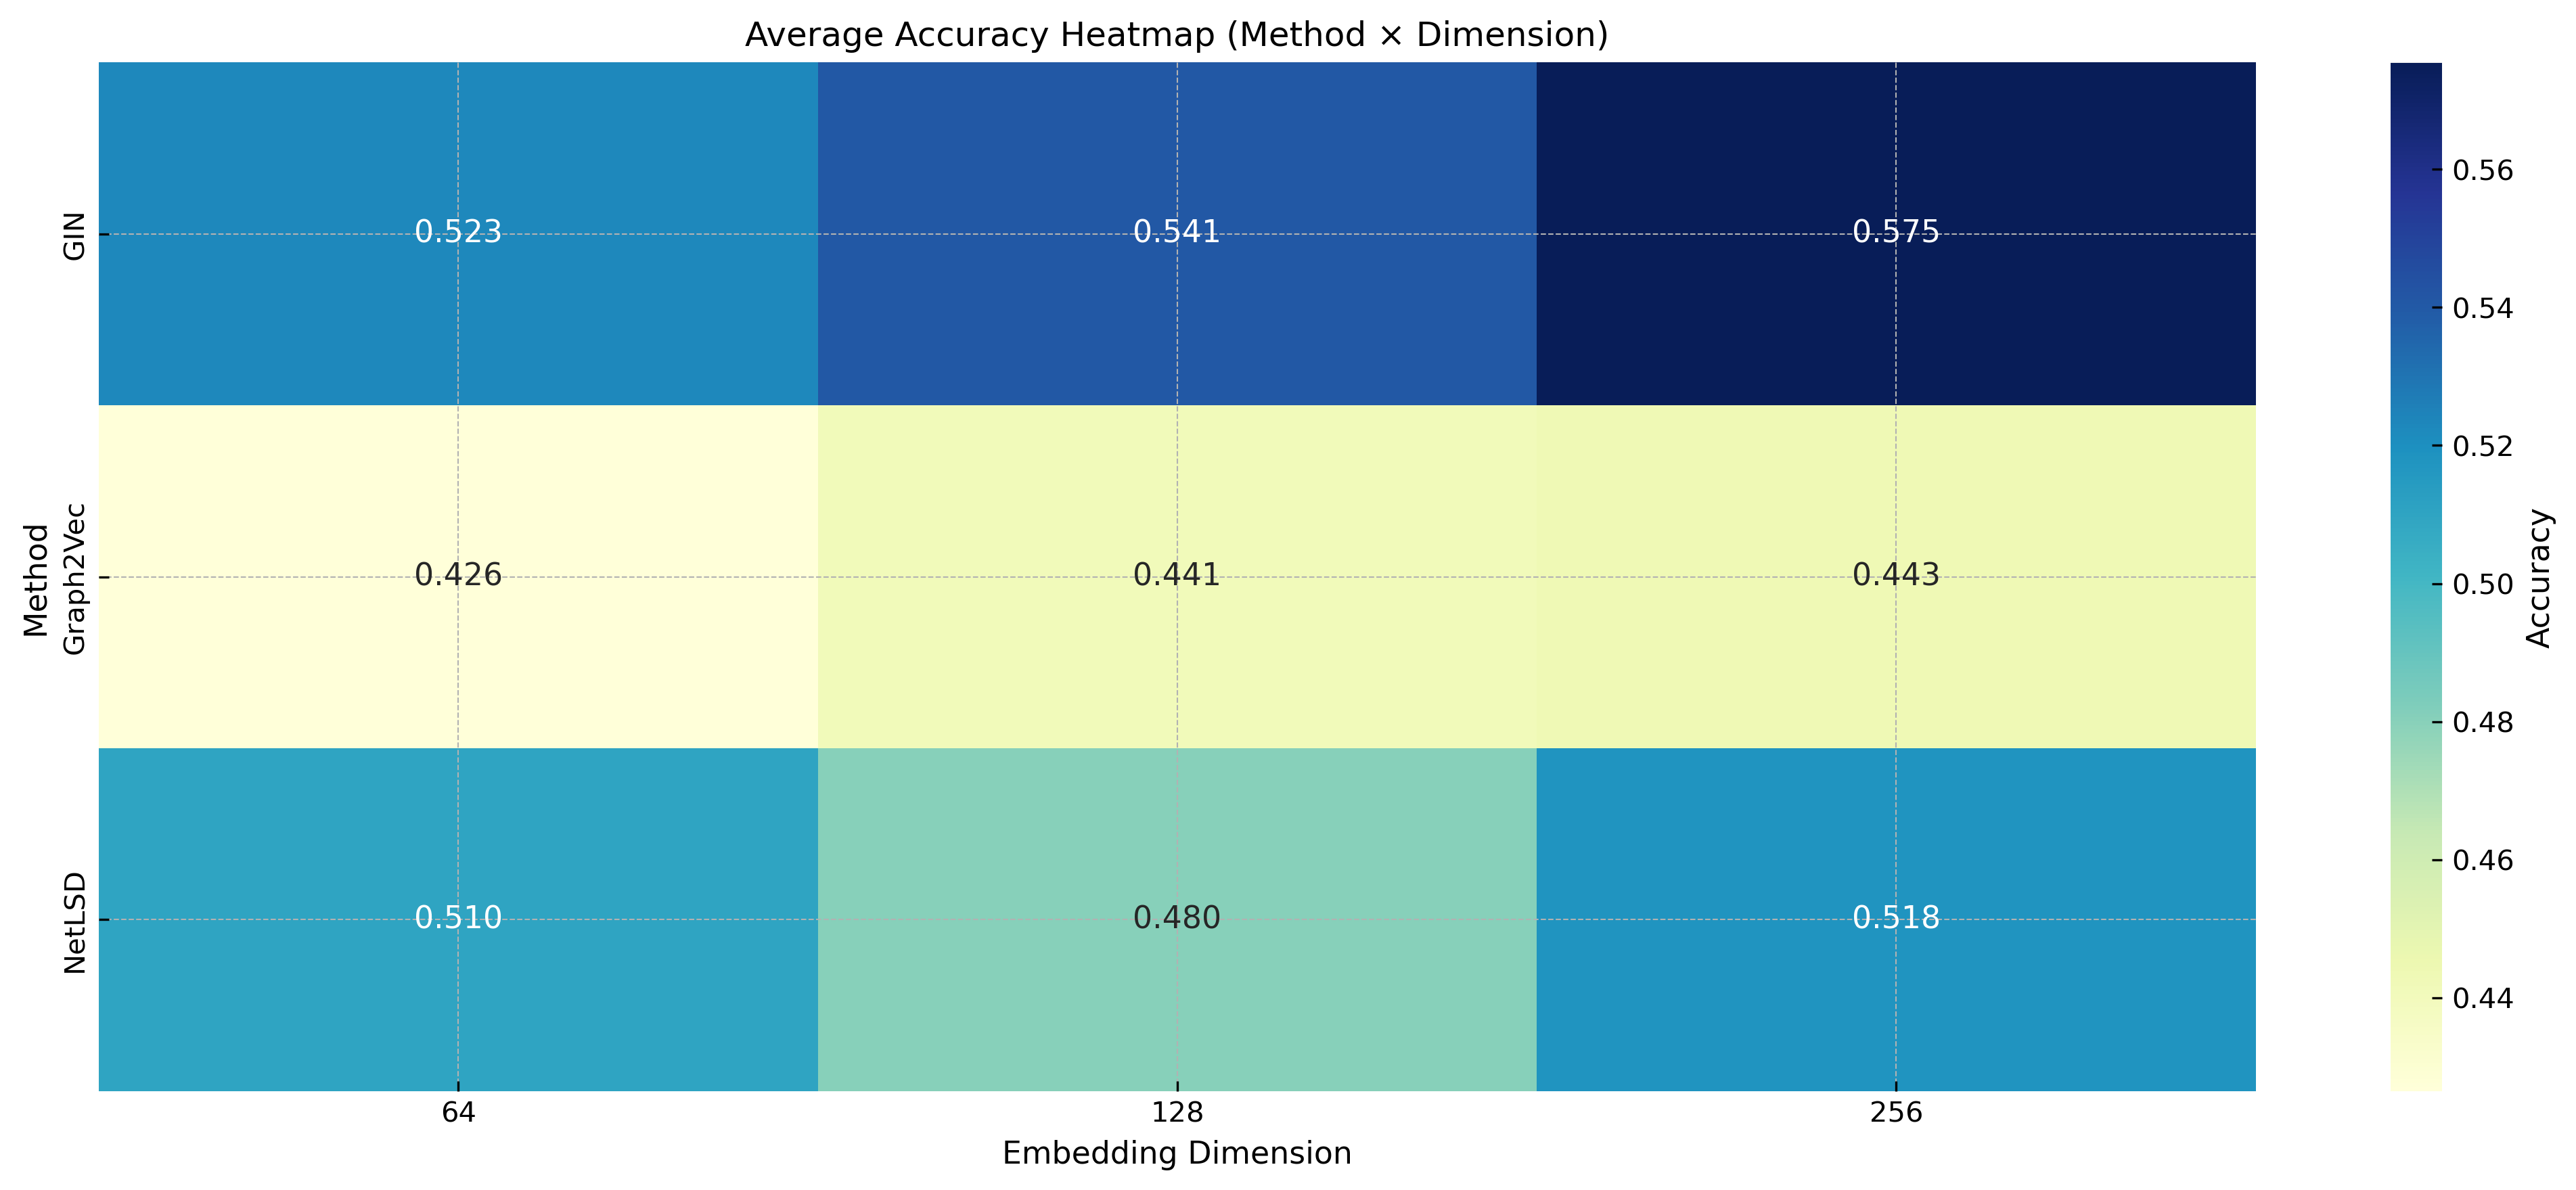
\includegraphics[width=\linewidth]{figures/HEATMAP_AVG_accuracy_bef.png}
    \caption{Average accuracy heatmap across methods and embedding dimensions.}
    \label{fig:heatmap}
\end{figure}

\begin{figure}[t]
    \centering
    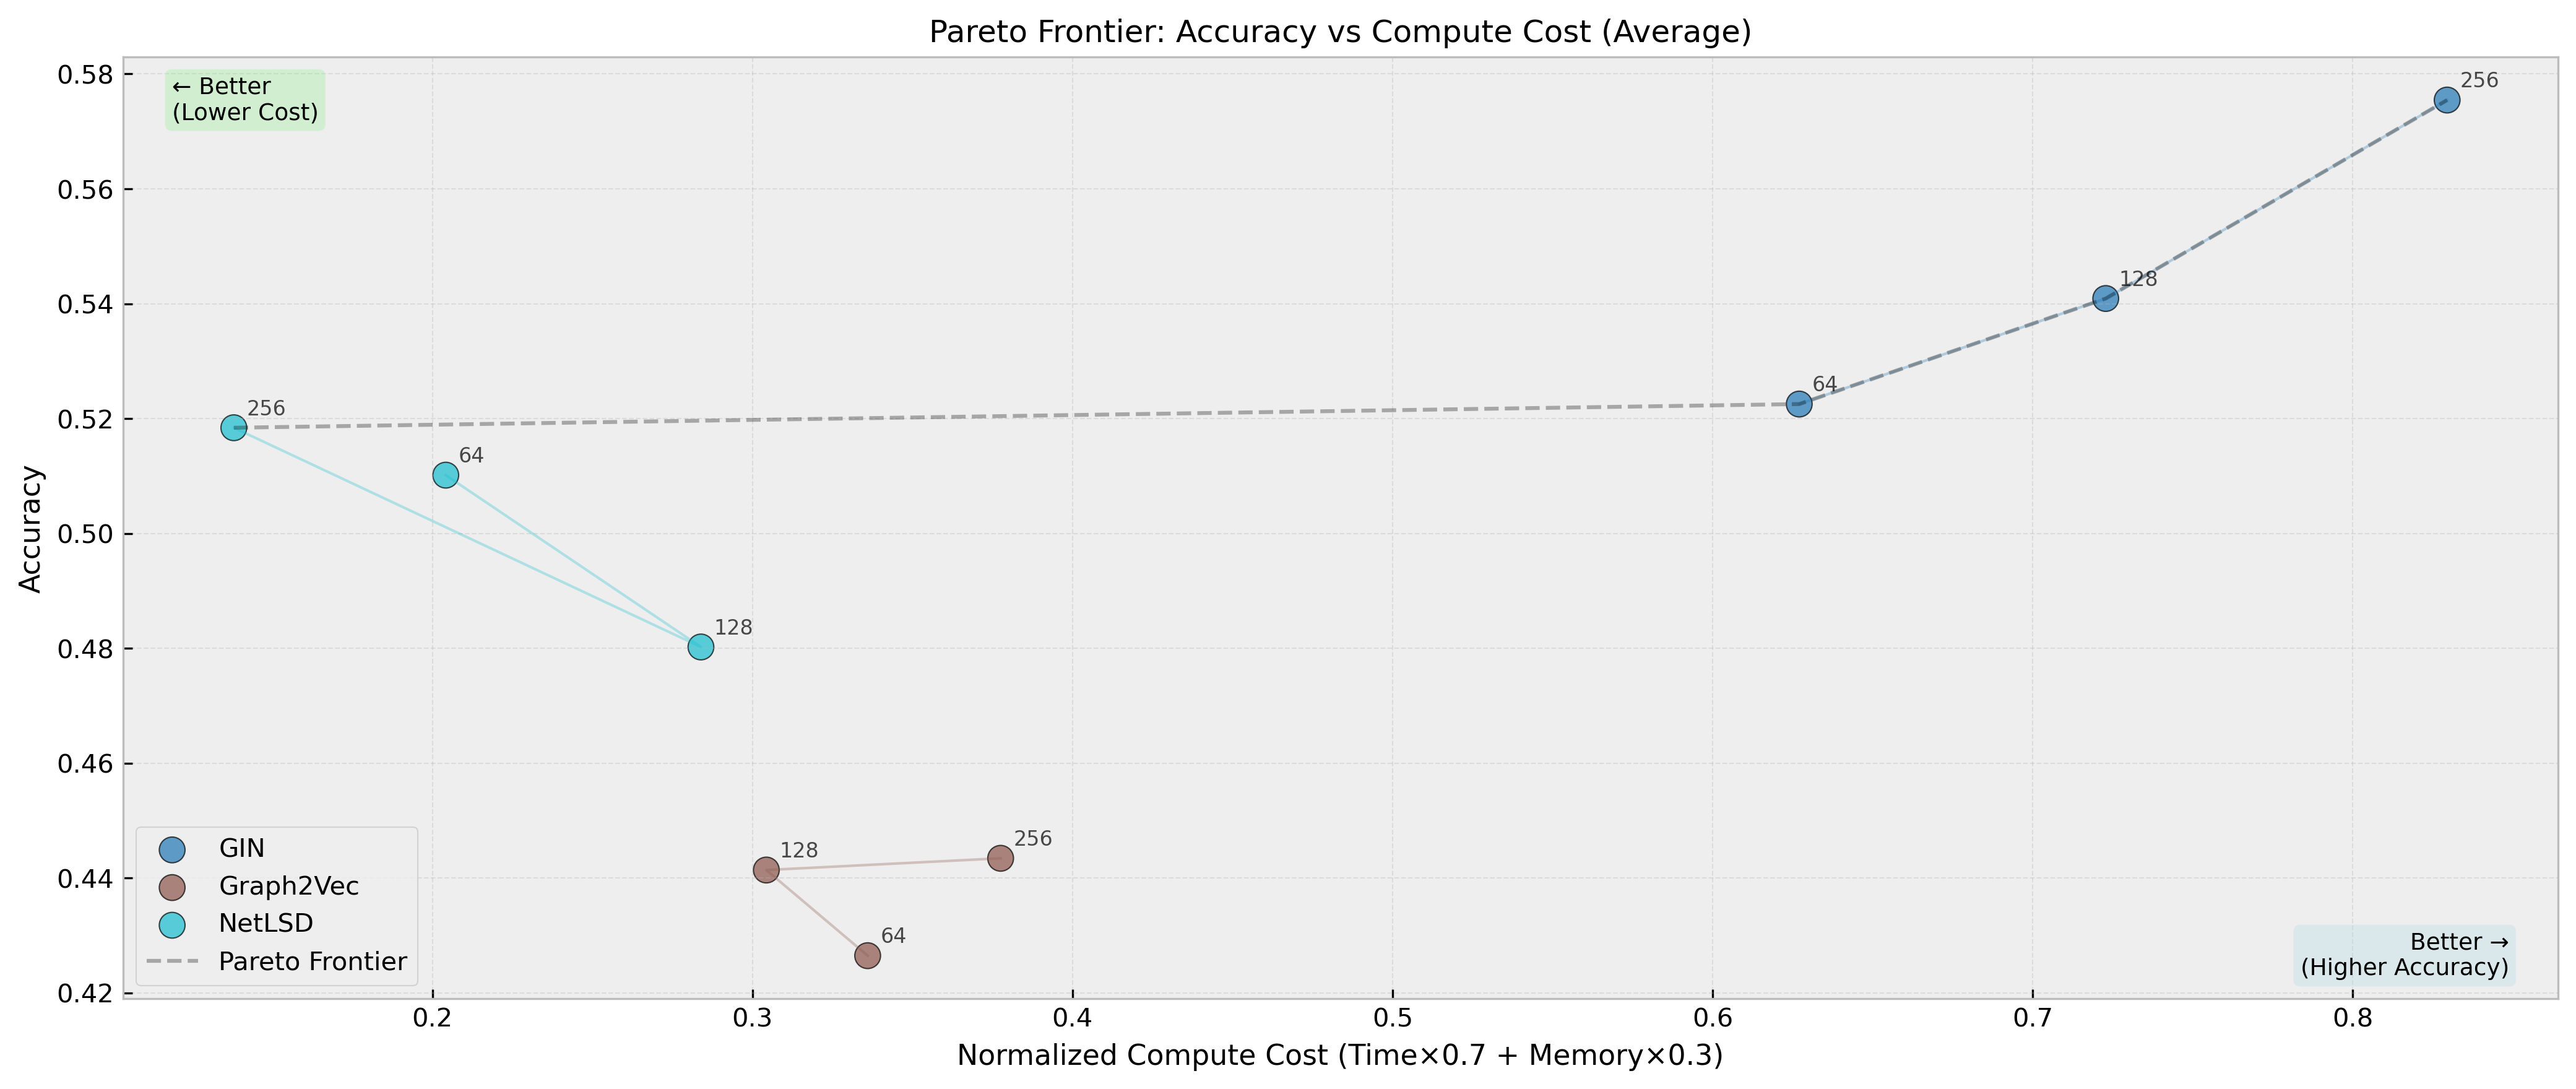
\includegraphics[width=\linewidth]{figures/PARETO_AVG_acc_vs_compute_cost_bef.png}
    \caption{Pareto frontier illustrating the trade-off between accuracy and normalized compute cost.}
    \label{fig:pareto}
\end{figure}

\begin{figure*}[t]
    \centering
    \begin{subfigure}{0.32\textwidth}
        \centering
        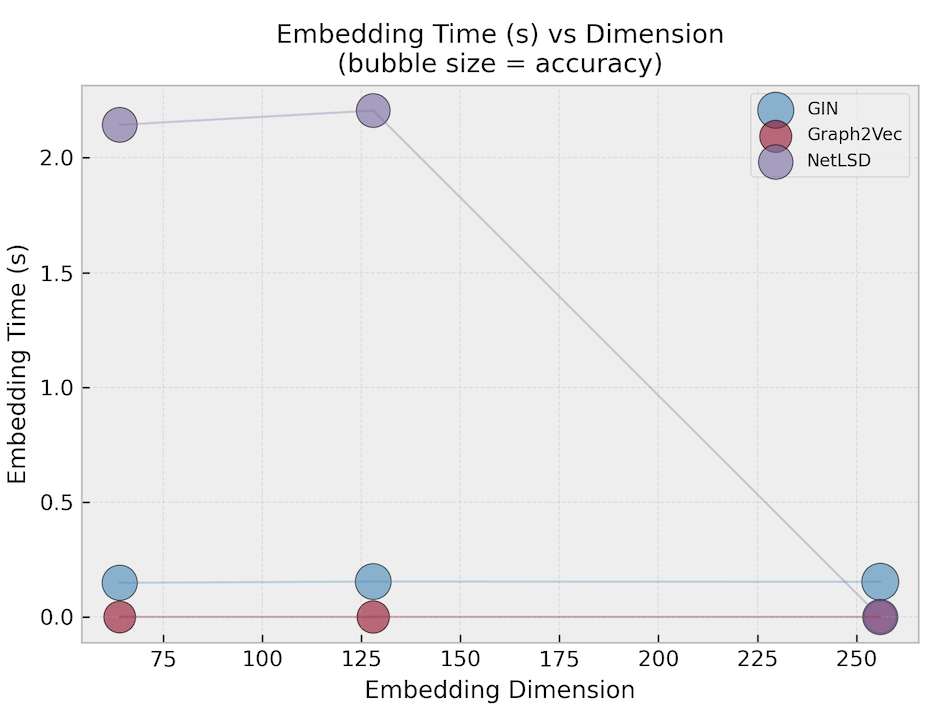
\includegraphics[width=\linewidth]{figures/gen_bef.png}
        \caption{Embedding time}
        \label{fig:embed_time}
    \end{subfigure}
    \hfill
    \begin{subfigure}{0.32\textwidth}
        \centering
        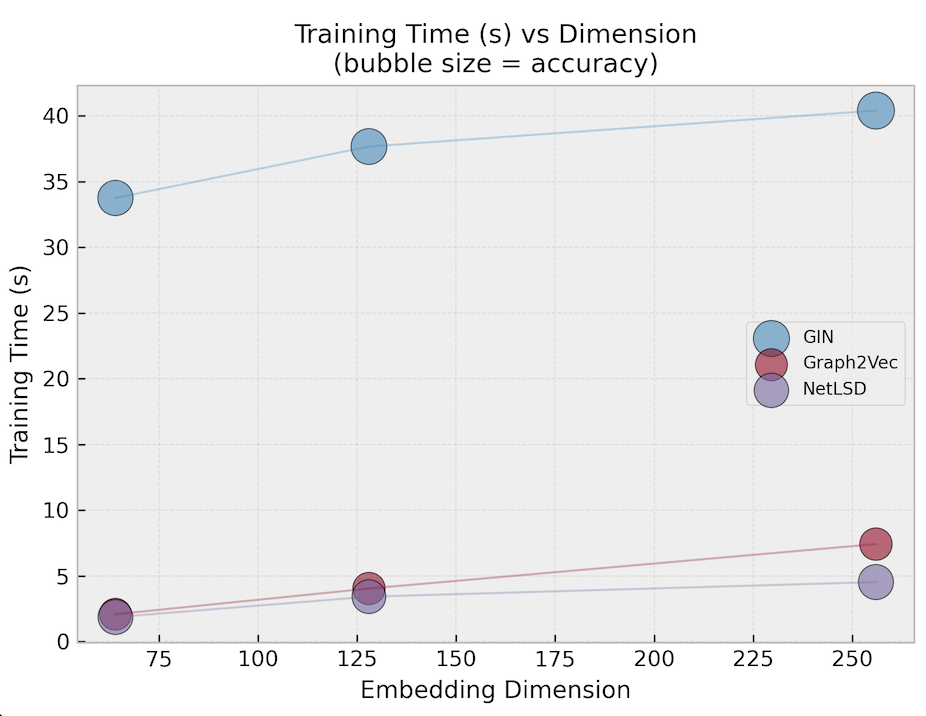
\includegraphics[width=\linewidth]{figures/train_bef.png}
        \caption{Training time}
        \label{fig:train_time}
    \end{subfigure}
    \hfill
    \begin{subfigure}{0.32\textwidth}
        \centering
        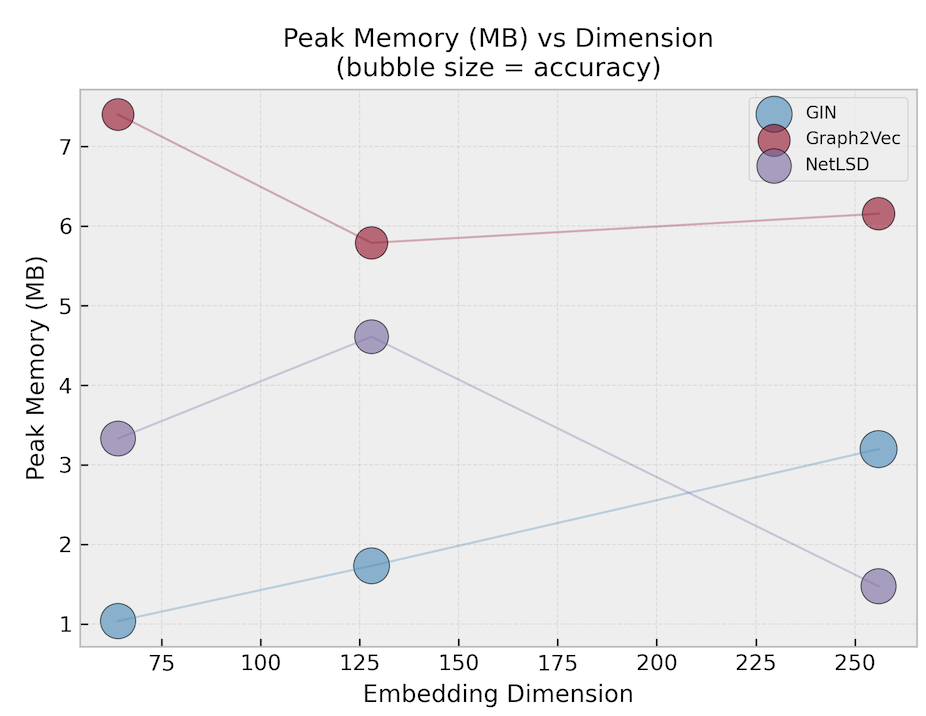
\includegraphics[width=\linewidth]{figures/mem_bef.png}
        \caption{Peak memory}
        \label{fig:peak_mem}
    \end{subfigure}

    \caption{Compute cost components as a function of embedding dimension. Bubble size indicates average accuracy.}
    \label{fig:cost_breakdown}
\end{figure*}



% \begin{figure}[t]
%     \centering
%     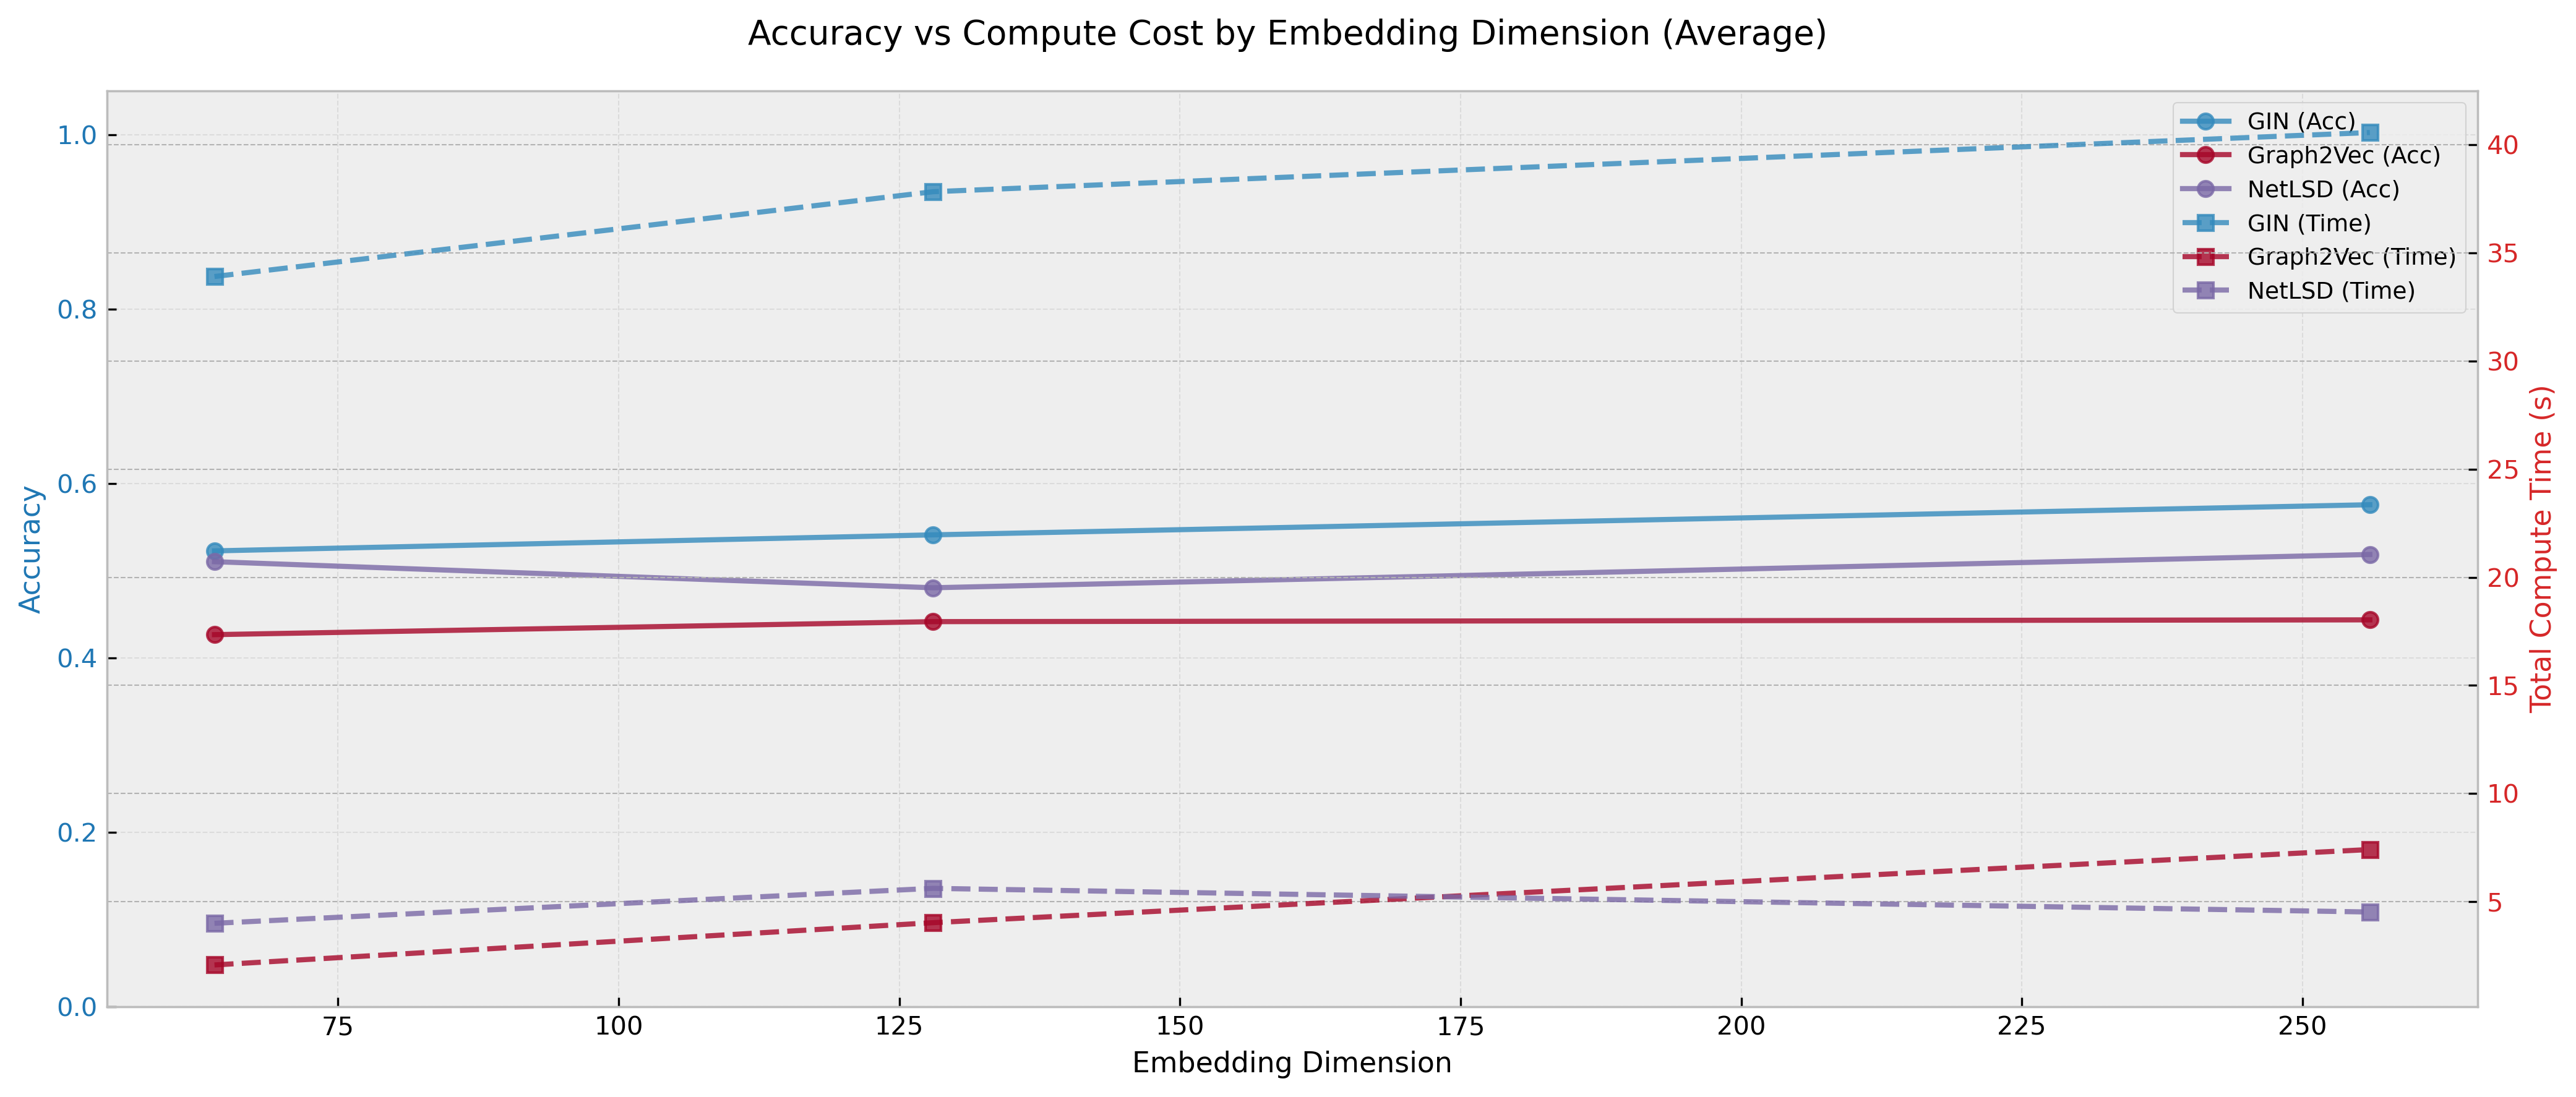
\includegraphics[width=\linewidth]{figures/DUAL_AVG_acc_vs_compute_cost_bef.png}
%     \caption{Accuracy and total compute cost versus embedding dimension (averaged across datasets).}
%     \label{fig:acc_vs_cost}
% \end{figure}



The experimental results reveal clear trade offs between classification 
accuracy and computational efficiency across GIN, Graph2Vec and NetLSD, 
as illustrated in Figures~\ref{fig:heatmap}-\ref{fig:cost_breakdown}. All figures are computed with the 
average results across the three dimensions and three datasets.
We chose these 3 images (from the 39 we generated for the classification section) to summarize and make our conclusions.

Figure~\ref{fig:heatmap} presents a heatmap of average accuracy across methods and embedding dimensions.
We can confirm that GIN consistently outperforms the other two methods across all dimensions.

The Pareto frontier in Figure~\ref{fig:pareto} highlights the balance between efficiency and performance.
NetLSD lies on the left most side of the optimal region, meaning that it achieves reasonable accuracy with minimal compute cost.
GIN dominates with its accuracy, but with a significantlt higher compute cost.
Graph2Vec is at the lower part of the graph, showing both lower accuracy from both other methods  and higher compute cost, than NetLSD.
From the same figure, we can see that GIN 
benefits monotonically from increased embedding dimensionality, 
achieving the highest average accuracy at 256 dimensions.
In contrast, Graph2Vec and NetLSD reach their peak accuracy at 128 dimensions,
beyond which performance declines, indicating diminishing returns with higher dimensions.

Figure~\ref{fig:cost_breakdown} breaks down the compute cost into embedding time, training time and peak memory usage.
Training time (Figure~\ref{fig:train_time}) is dominated by GIN and increases substantially with embedding dimension.
Embedding time (Figure~\ref{fig:embed_time}) is highest for NetLSD at lower dimensions 
due to its spectral computations but decreases at higher dim sizes.
Peak memory usage (Figure~\ref{fig:peak_mem}) is highest for Graph2Vec,
while NetLSD remains more memory efficient. 





\subsection{After Permutation}